\documentclass[a4paper]{article}

%%%%%%%% CREATE DOCUMENT STRUCTURE %%%%%%%%
%% Language and font encodings
\usepackage[polish]{babel}
\usepackage[utf8]{inputenc}
\usepackage[T1]{fontenc}
%\usepackage{subfig}

%% Sets page size and margins
\usepackage[a4paper,top=3cm,bottom=2cm,left=2cm,right=2cm,marginparwidth=1.75cm]{geometry}

%% Useful packages
\usepackage{amsmath}
\usepackage{graphicx}
\usepackage[colorinlistoftodos]{todonotes}
\usepackage{float}
\usepackage[colorlinks=true, allcolors=blue]{hyperref}
\usepackage{caption}
\usepackage{subcaption}
\usepackage{sectsty}
\usepackage{titling}
\usepackage{blindtext}
\usepackage[square,sort,comma,numbers]{natbib}
\usepackage[colorinlistoftodos]{todonotes}
\usepackage{xcolor}
\definecolor{darkgreen}{rgb}{0.0, 0.4, 0.0}

%%%%%%%% DOCUMENT %%%%%%%%
\begin{document}

%%%% Title Page
\begin{titlepage}

\newcommand{\HRule}{\rule{\linewidth}{0.5mm}}
\center

\textsc{\LARGE Politechnika Krakowska}\\[1cm]

\textsc{\Large Bezpieczeństwo i Hardening Systemów Operacyjnych}\\[0.2cm]
\HRule \\[0.8cm]
{ \huge \bfseries Szyfrowanie danych w systemie Linux: analiza porównawcza LUKS, eCryptfs i fscrypt }\\[0.7cm]
\HRule \\[2cm]
\Large Jakub Mikusek\\[1.5cm]
{\large \today}\\[5cm]
% \includegraphics[width=0.5\textwidth]{PK_logo.png}\\[1cm]
\vfill
\end{titlepage}

\section{Wprowadzenie}

W ramach projektu stworzony został benchmark porównujący wydajność trzech sposobów szyfrowania
plików w systemach Linux, porównanie oraz sposób działania każdego z rozwiązań oraz
rekomendacje dla scenariuszy użycia.

Do testów porównawczych został dodatkowo zmierzony czas wykonywania operacji wejścia/wyjścia
(I/O) dla niezaszyfrowanych plików, aby w wynikach uwzględnić narzut każdej z metod szyfrowania.

\section{fscrypt}
W przeciwieństwie do dm-crypt (LUKS), fscrypt działa na poziomie systemu plików. Dzięki temu
wykorzystanie tego mechanizmu szyfrowania pozwala na niezależne szyfrowanie pojedynczych
plików. Taki sposób szyfrowania daje większą elastyczność oraz w przypadku urządzeń
wykorzystywanych przez wielu użytkowników, pozwala na logiczny podział odstępu do
poszczególnych plików.

Bezpośrednie zintegrowanie fscrypt do systemu plików pozwala na lepszą wydajność,
w porównaniu do eCryptfs, gdzie jest on dodatkową abstrakcją na system plików. Takie
podejście pozwala na szybszy dostęp do zawartości plików, bez konieczności przechowywania
w pamięci podręcznej zaszyfrowanej oraz odszyfrowanej wersji pliku. Dodatkową zaletą
używania fscrypt w stosunku do eCryptfs jest brak narzutu związanego z metadanymi w nazwie
pliku, co pozwala na wykorzystanie pełnych 255 bajtów na nazwę pliku.



\section{Testy wydajnościowe}
Testy wydajnościowe obejmują wykorzystanie prostego polecenia \texttt{dd}, pozwalającego na
kopiowanie z oraz do plików specyfikując ilość bajtów w ramach pojedynczej operacji.
Bardziej szczegółowe testy zostały przeprowadzone przy pomocy \texttt{fio}, który pozwala
symulowanie operacji wejścia/wyjścia na podstawie zadanych parametrów.

Do automatyzacji wykonywania testów zostały stworzone dwa skrypty przy użyciu języka python3
(\textit{benchmark\_dd.py} oraz \textit{benchmark\_fio.py}). Pozwalają one dzięki
parametrom wykonania na dostosowanie ilości wykonywanych testów.

\subsection{Testy wykorzystujące \texttt{dd}}
Polecenie \texttt{dd} pozwala na proste operacje kopiowania danych pomiędzy plikami,
na podstawie zadanego rozmiaru bloku w bajtach, opcja \texttt{bs=}, oraz ilości kopiowanych
danych dzięki opcji \texttt{count=}. W połączeniu z urządzeniem \textit{/dev/urandom},
\texttt{dd} pozwala na przetestowanie przepustowości oraz szybkości kopiowania losowych danych
do plików zaszyfrowanych wybraną metodą. Natomiast wykorzystując \textit{/dev/null},
\texttt{dd} umożliwia przetestowanie szybkości kopiowania danych z plików.


\subsubsection{Wyniki uzyskane w ramach testów przy użyciu \texttt{dd}}

\begin{table}[H]
    \centering
    \begin{tabular}{|l|l|r|}
        \hline
        Mechanism & Operation & Speed (MBs) \\
        \hline
        Raw I/O [4K] & WRITE & 124.6 \\
        Raw I/O [4K] & READ & 124.4 \\
        Raw I/O [512K] & WRITE & 381.2 \\
        Raw I/O [512K] & READ & 474.9 \\
        Raw I/O [1M] & WRITE & 398.8 \\
        Raw I/O [1M] & READ & 848.5 \\
        Raw I/O [4M] & WRITE & 414.8 \\
        Raw I/O [4M] & READ & 1008.5 \\
        LUKS [4K] & WRITE & 103.39 \\
        LUKS [4K] & READ & 98.68 \\
        LUKS [512K] & WRITE & 351.1 \\
        LUKS [512K] & READ & 363.2 \\
        LUKS [1M] & WRITE & 387.1 \\
        LUKS [1M] & READ & 647.4 \\
        LUKS [4M] & WRITE & 420.3 \\
        LUKS [4M] & READ & 699.3 \\
        eCryptfs [4K] & WRITE & 94.18 \\
        eCryptfs [4K] & READ & 110.63 \\
        eCryptfs [512K] & WRITE & 210.7 \\
        eCryptfs [512K] & READ & 139.8 \\
        eCryptfs [1M] & WRITE & 218.5 \\
        eCryptfs [1M] & READ & 139.2 \\
        eCryptfs [4M] & WRITE & 217.5 \\
        eCryptfs [4M] & READ & 137.9 \\
        fscrypt [4K] & WRITE & 136.0 \\
        fscrypt [4K] & READ & 103.34 \\
        fscrypt [512K] & WRITE & 346.0 \\
        fscrypt [512K] & READ & 381.0 \\
        fscrypt [1M] & WRITE & 357.5 \\
        fscrypt [1M] & READ & 715.0 \\
        fscrypt [4M] & WRITE & 404.4 \\
        fscrypt [4M] & READ & 820.1 \\
        \hline
    \end{tabular}
    \caption{Tabela wyników operacji wyjścia (READ) oraz wejścia (WRITE) do plików w ramach
    różnych mechanizmów szyfrowania danych.}
    \label{tab:dd_results}
\end{table}

\begin{figure}[H]
    \centering
    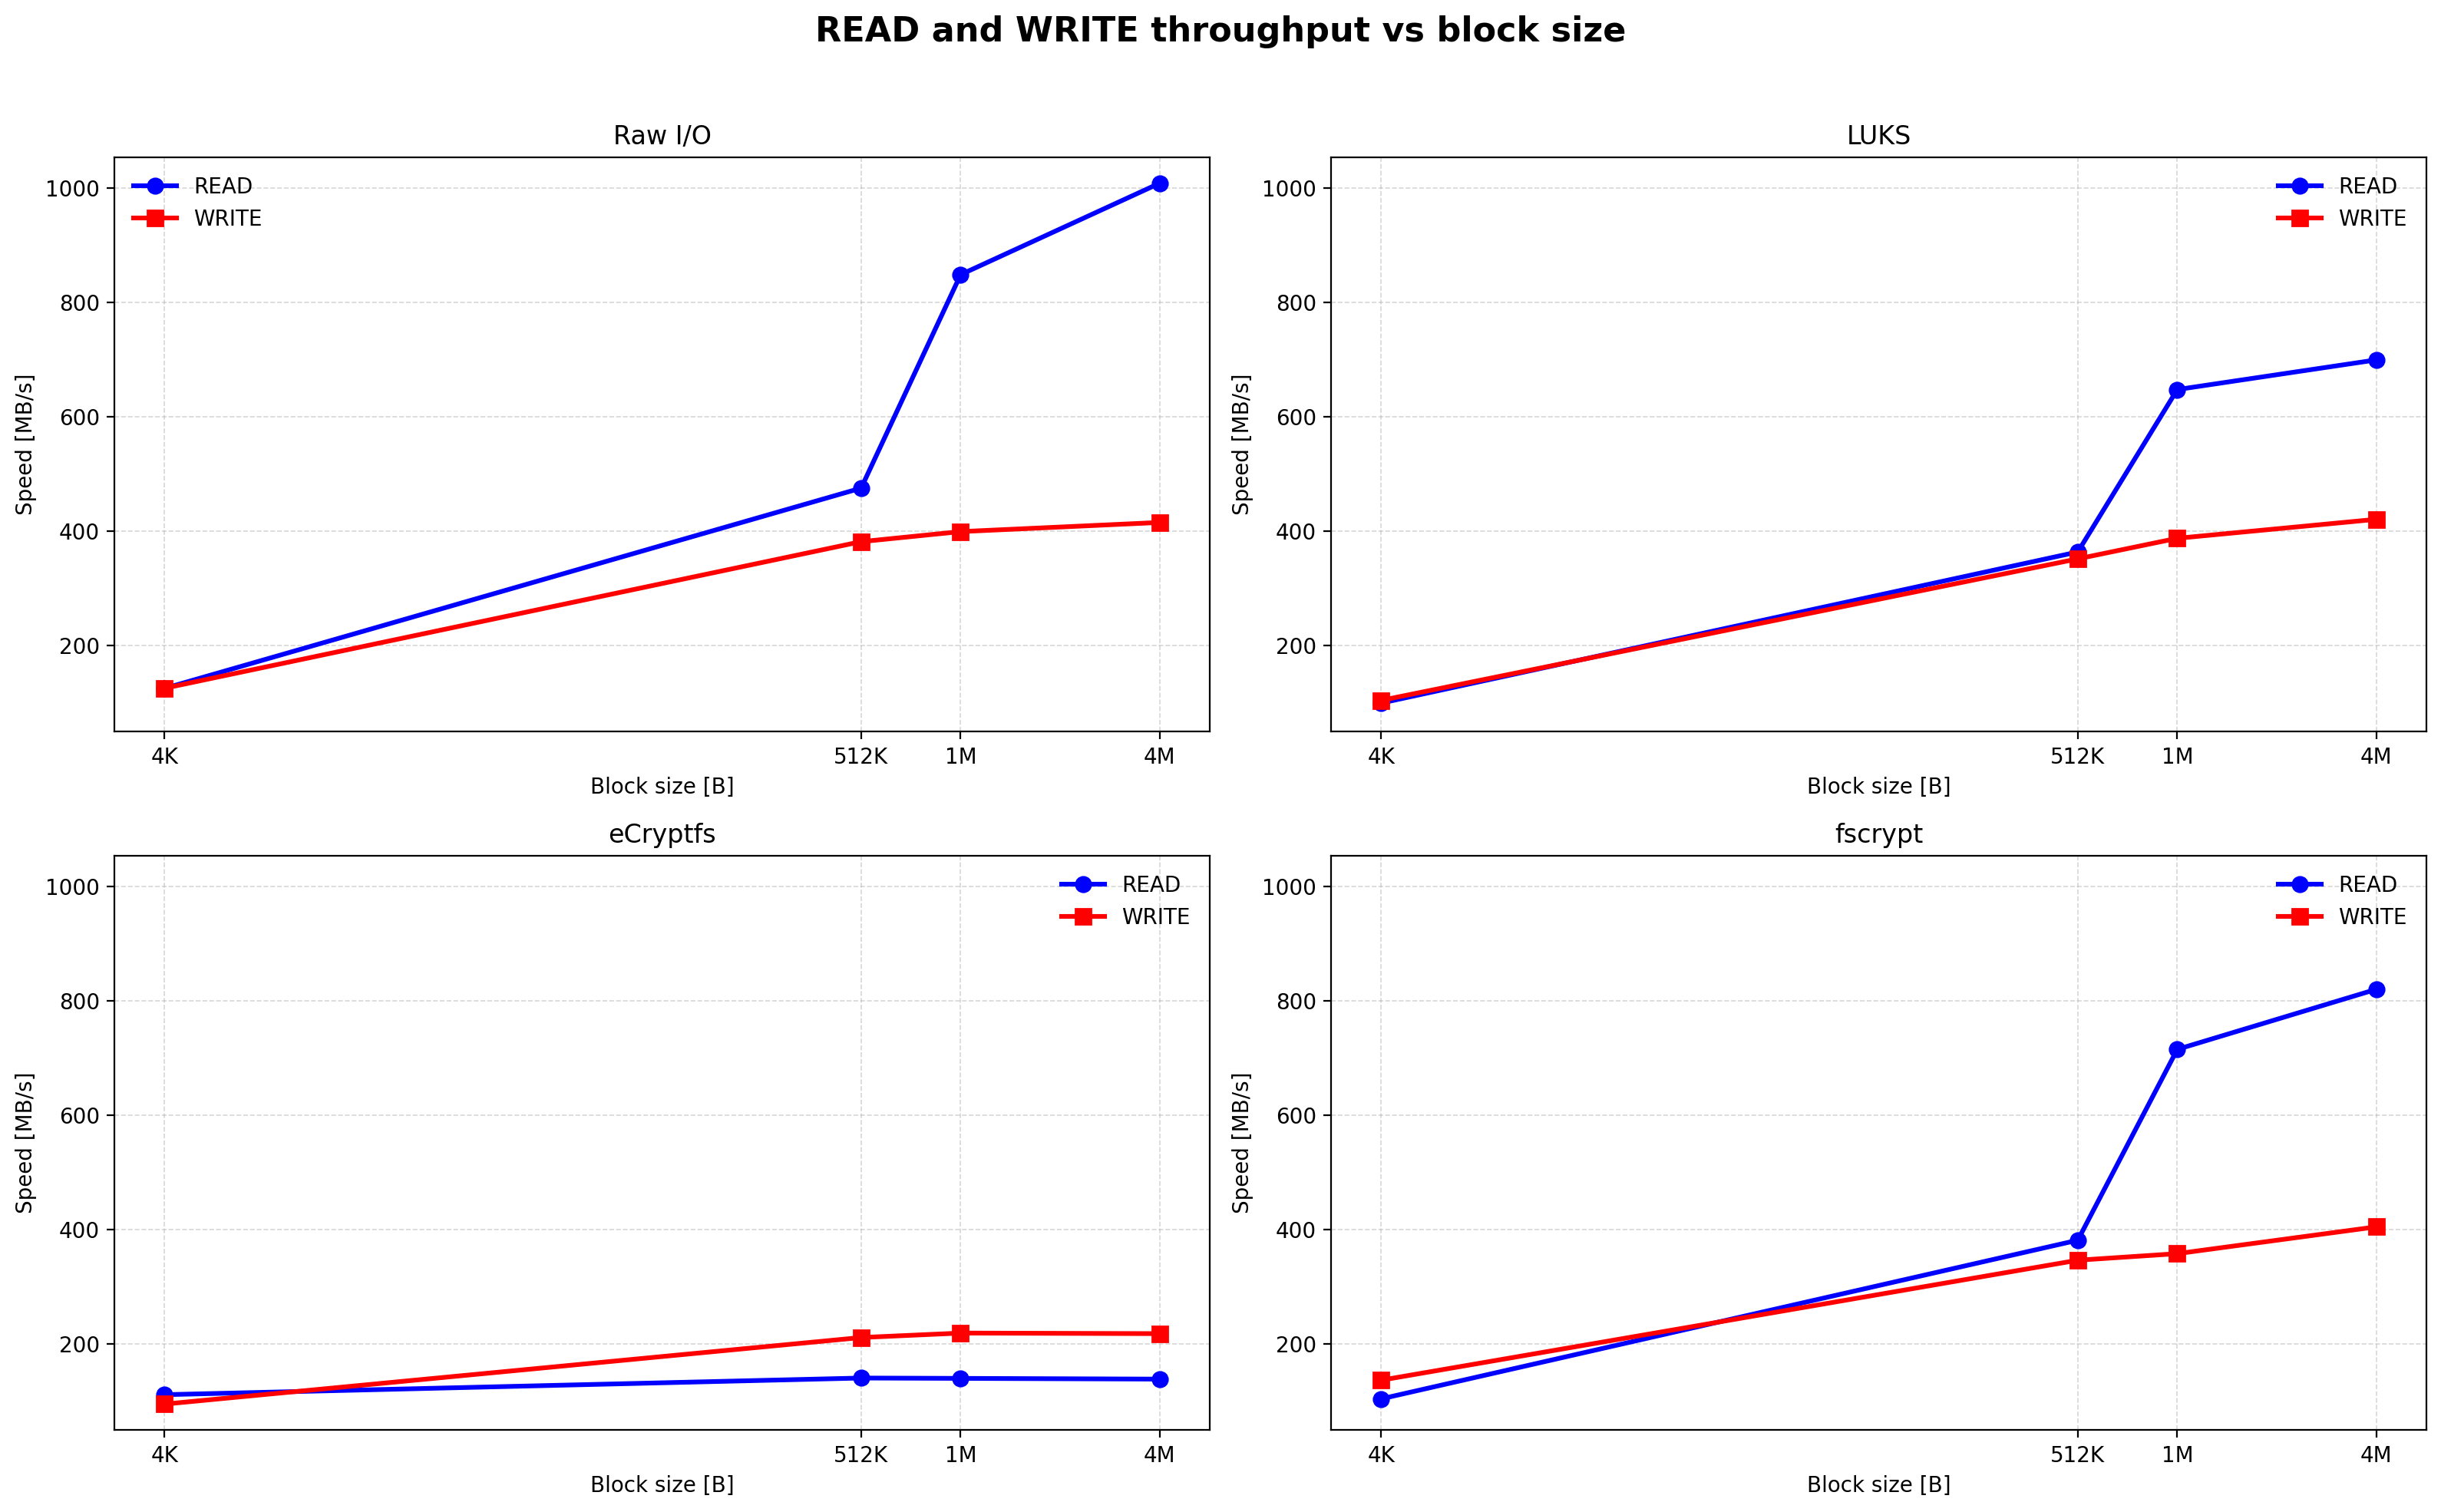
\includegraphics[width=\linewidth]{dd_final_plot.png}
    \caption{Wykres zależności wielkości bloku w bajtach do szybkości operacji kopiowania z
    oraz do szyfrowanych plików różnymi mechanizmami.}
    \label{fig:dd_results}
\end{figure}

\subsubsection{Wnioski}

Na podstawie surowych danych z tabeli \eqref{tab:dd_results} oraz wykresu \eqref{fig:dd_results},
można stwierdzić, że najlepsze wyniki dla czytania danych osiąga brak szyfrowania.
LUKS oraz fscrypt osiągają porównywalne wyniki, co wynika ze sposobu szyfrowania, gdzie
dla LUKS szyfrowana jest cała partycja, oraz dla fscrypt, gdzie szyfrowane są katalogi, co
powoduje niewielki narzut na szybkość odczytywania danych w porównaniu do braku szyfrowania.
W przypadku eCryptfs, gdzie szyfrowanie odbywa się per-plik, narzut na operacje czytania
jest największy ze wszystkich porównywanych mechanizmów.

Mechanizmy LUKS oraz fscrypt w porównaniu do braku szyfrowania nie powodują dodatkowego narzutu,
związanego z zapisem danych do plików. Natomiast podobnie jak dla operacji odczytu,
eCryptfs powoduje zauważalny spadek w szybkości zapisów w porównaniu do pozostałych metod
szyfrowania.


\subsection{Testy wykorzystujące \texttt{fio}}
Narzędzie \texttt{fio} pozwala na bardziej złożone testy wydajności wybranego mechanizmu
szyfrowania plików dzięki jednoczesnym operacjom wejścia i wyjścia oraz na między innymi
wybranie sposobu kopiowania plików (sekwencyjne \& losowe). W ramach benchmarków
przetestowano kopiowanie sekwencyjne i losowe bloków o różnej wielkości oraz
jednoczesne wykonywanie operacji I/O o równym (50/50) rozłożeniu oraz nierównomiernym (70/30).


\begin{table}[H]
    \centering
    \small
    \begin{tabular}{|l|l|r|r|}
        \hline
        Mechanism & Test & Read I/OPS & Write I/OPS \\
        \hline
        Raw I/O & Sequential write 4k & 0 & 5450 \\
        Raw I/O & Sequential read 4k & 6358 & 0 \\
        Raw I/O & Sequential write 1M & 0 & 1370 \\
        Raw I/O & Sequential read 1M & 1207 & 0 \\
        Raw I/O & Random write 4k & 0 & 3201 \\
        Raw I/O & Random read 4k & 3533 & 0 \\
        Raw I/O & Random write 1M & 0 & 1349 \\
        Raw I/O & Random read 1M & 1193 & 0 \\
        Raw I/O & Mixed 70\%R/30\%W 1M & 839 & 360 \\
        Raw I/O & Mixed 50\%R/50\%W 1M & 605 & 604 \\
        LUKS & Sequential write 4k & 0 & 17167 \\
        LUKS & Sequential read 4k & 6047 & 0 \\
        LUKS & Sequential write 1M & 0 & 1305 \\
        LUKS & Sequential read 1M & 1177 & 0 \\
        LUKS & Random write 4k & 0 & 2853 \\
        LUKS & Random read 4k & 3416 & 0 \\
        LUKS & Random write 1M & 0 & 1343 \\
        LUKS & Random read 1M & 1214 & 0 \\
        LUKS & Mixed 70\%R/30\%W 1M & 894 & 383 \\
        LUKS & Mixed 50\%R/50\%W 1M & 626 & 633 \\
        eCryptfs & Sequential write 4k  & 0 & 114356 \\
        eCryptfs & Sequential read 4k  & 910493 & 0 \\
        eCryptfs & Sequential write 1M  & 0 & 464 \\
        eCryptfs & Sequential read 1M  & 2264 & 0 \\
        eCryptfs & Random write 4k  & 0 & 100559 \\
        eCryptfs & Random read 4k  & 1963 & 0 \\
        eCryptfs & Random write 1M  & 0 & 474 \\
        eCryptfs & Random read 1M  & 17937 & 0 \\
        eCryptfs & Mixed 70\%R/30\%W 1M  & 1108 & 471 \\
        eCryptfs & Mixed 50\%R/50\%W 1M  & 481 & 490 \\
        fscrypt & Sequential write 4k & 0 & 261970 \\
        fscrypt & Sequential read 4k & 2893650 & 0 \\
        fscrypt & Sequential write 1M & 0 & 2105 \\
        fscrypt & Sequential read 1M & 19955 & 0 \\
        fscrypt & Random write 4k & 0 & 280132 \\
        fscrypt & Random read 4k & 2222 & 0 \\
        fscrypt & Random write 1M & 0 & 2459 \\
        fscrypt & Random read 1M & 20678 & 0 \\
        fscrypt & Mixed 70\%R/30\%W 1M & 4330 & 1854 \\
        fscrypt & Mixed 50\%R/50\%W 1M & 1883 & 1878 \\
        \hline
    \end{tabular}
    \caption{Tabela wyników w podziale na operacje I/O (wejścia/wyjścia) na sekundę.}
    \label{tab:fio_iops}
\end{table}

\begin{table}[H]
    \centering
    \small
    \begin{tabular}{|l|l|r|r|}
        \hline
        Mechanism & Test & Read BW MB/s & Write BW MB/s \\
        \hline
        Raw I/O & Sequential write 4k & 0.00 & 21.29 \\
        Raw I/O & Sequential read 4k & 24.83 & 0.00 \\
        Raw I/O & Sequential write 1M & 0.00 & 1369.96 \\
        Raw I/O & Sequential read 1M & 1207.32 & 0.00 \\
        Raw I/O & Random write 4k & 0.00 & 12.50 \\
        Raw I/O & Random read 4k & 13.80 & 0.00 \\
        Raw I/O & Random write 1M & 0.00 & 1349.27 \\
        Raw I/O & Random read 1M & 1193.10 & 0.00 \\
        Raw I/O & Mixed 70\%R/30\%W 1M & 839.14 & 360.00 \\
        Raw I/O & Mixed 50\%R/50\%W 1M & 604.72 & 603.82 \\
        LUKS & Sequential write 4k & 0.00 & 67.06 \\
        LUKS & Sequential read 4k & 23.62 & 0.00 \\
        LUKS & Sequential write 1M & 0.00 & 1305.19 \\
        LUKS & Sequential read 1M & 1176.68 & 0.00 \\
        LUKS & Random write 4k & 0.00 & 11.14 \\
        LUKS & Random read 4k & 13.34 & 0.00 \\
        LUKS & Random write 1M & 0.00 & 1342.88 \\
        LUKS & Random read 1M & 1213.72 & 0.00 \\
        LUKS & Mixed 70\%R/30\%W 1M & 893.97 & 383.48 \\
        LUKS & Mixed 50\%R/50\%W 1M & 626.13 & 632.52 \\
        eCryptfs & Sequential write 4k  & 0.00 & 446.70 \\
        eCryptfs & Sequential read 4k  & 3556.61 & 0.00 \\
        eCryptfs & Sequential write 1M  & 0.00 & 464.01 \\
        eCryptfs & Sequential read 1M  & 2263.98 & 0.00 \\
        eCryptfs & Random write 4k  & 0.00 & 392.81 \\
        eCryptfs & Random read 4k  & 7.67 & 0.00 \\
        eCryptfs & Random write 1M  & 0.00 & 473.64 \\
        eCryptfs & Random read 1M  & 17937.47 & 0.00 \\
        eCryptfs & Mixed 70\%R/30\%W 1M  & 1108.41 & 470.83 \\
        eCryptfs & Mixed 50\%R/50\%W 1M  & 481.25 & 489.98 \\
        fscrypt & Sequential write 4k & 0.00 & 1023.32 \\
        fscrypt & Sequential read 4k & 11303.32 & 0.00 \\
        fscrypt & Sequential write 1M & 0.00 & 2105.25 \\
        fscrypt & Sequential read 1M & 19955.23 & 0.00 \\
        fscrypt & Random write 4k & 0.00 & 1094.27 \\
        fscrypt & Random read 4k & 8.68 & 0.00 \\
        fscrypt & Random write 1M & 0.00 & 2458.55 \\
        fscrypt & Random read 1M & 20677.51 & 0.00 \\
        fscrypt & Mixed 70\%R/30\%W 1M & 4330.03 & 1853.64 \\
        fscrypt & Mixed 50\%R/50\%W 1M & 1883.16 & 1877.72 \\
        \hline
    \end{tabular}
    \caption{Tabela wyników przepustowości osiągana przez poszczególne mechanizmy szyfrowania.}
    \label{tab:fio_bw}
\end{table}

\begin{table}[H]
    \centering
    \small
    \begin{tabular}{|l|l|r|r|}
        \hline
        Mechanism & Test & Read latency us & Write latency us \\
        \hline
        Raw I/O & Sequential write 4k & 0.0 & 11736.5 \\
        Raw I/O & Sequential read 4k & 10060.9 & 0.0 \\
        Raw I/O & Sequential write 1M & 0.0 & 46686.5 \\
        Raw I/O & Sequential read 1M & 52939.3 & 0.0 \\
        Raw I/O & Random write 4k & 0.0 & 19985.0 \\
        Raw I/O & Random read 4k & 18106.7 & 0.0 \\
        Raw I/O & Random write 1M & 0.0 & 47402.1 \\
        Raw I/O & Random read 1M & 53592.4 & 0.0 \\
        Raw I/O & Mixed 70\%R/30\%W 1M & 38852.4 & 87042.6 \\
        Raw I/O & Mixed 50\%R/50\%W 1M & 33539.9 & 72302.3 \\
        LUKS & Sequential write 4k & 0.0 & 3726.9 \\
        LUKS & Sequential read 4k & 10576.6 & 0.0 \\
        LUKS & Sequential write 1M & 0.0 & 49017.9 \\
        LUKS & Sequential read 1M & 54339.2 & 0.0 \\
        LUKS & Random write 4k & 0.0 & 22427.3 \\
        LUKS & Random read 4k & 18725.6 & 0.0 \\
        LUKS & Random write 1M & 0.0 & 47646.6 \\
        LUKS & Random read 1M & 52681.0 & 0.0 \\
        LUKS & Mixed 70\%R/30\%W 1M & 40498.3 & 72345.9 \\
        LUKS & Mixed 50\%R/50\%W 1M & 32301.8 & 69139.9 \\
        eCryptfs & Sequential write 4k  & 0.0 & 558.9 \\
        eCryptfs & Sequential read 4k  & 69.7 & 0.0 \\
        eCryptfs & Sequential write 1M  & 0.0 & 137588.8 \\
        eCryptfs & Sequential read 1M  & 28107.0 & 0.0 \\
        eCryptfs & Random write 4k  & 0.0 & 605.6 \\
        eCryptfs & Random read 4k  & 32573.9 & 0.0 \\
        eCryptfs & Random write 1M  & 0.0 & 128480.3 \\
        eCryptfs & Random read 1M  & 3542.3 & 0.0 \\
        eCryptfs & Mixed 70\%R/30\%W 1M  & 38011.3 & 45616.1 \\
        eCryptfs & Mixed 50\%R/50\%W 1M  & 61994.8 & 69244.7 \\
        fscrypt & Sequential write 4k & 0.0 & 243.9 \\
        fscrypt & Sequential read 4k & 21.9 & 0.0 \\
        fscrypt & Sequential write 1M & 0.0 & 29404.3 \\
        fscrypt & Sequential read 1M & 3203.1 & 0.0 \\
        fscrypt & Random write 4k & 0.0 & 182.2 \\
        fscrypt & Random read 4k & 28784.9 & 0.0 \\
        fscrypt & Random write 1M & 0.0 & 25881.3 \\
        fscrypt & Random read 1M & 3088.4 & 0.0 \\
        fscrypt & Mixed 70\%R/30\%W 1M & 10190.6 & 10668.3 \\
        fscrypt & Mixed 50\%R/50\%W 1M & 17036.1 & 16927.0 \\
        \hline
    \end{tabular}
    \caption{Tabela wyników opóźnienia odczytu i zapisu mierzone w mikrosekundach.}
    \label{tab:fio_latency}
\end{table}

\begin{table}[H]
    \centering
    \small
    \begin{tabular}{|l|l|r|r|}
        \hline
        Mechanism & Test & CPU user \% & CPU sys \% \\
        \hline
        Raw I/O & Sequential write 4k & 0.3 & 47.2 \\
        Raw I/O & Sequential read 4k & 0.3 & 57.2 \\
        Raw I/O & Sequential write 1M & 1.1 & 41.8 \\
        Raw I/O & Sequential read 1M & 0.2 & 31.2 \\
        Raw I/O & Random write 4k & 0.2 & 34.5 \\
        Raw I/O & Random read 4k & 0.2 & 26.5 \\
        Raw I/O & Random write 1M & 1.1 & 41.0 \\
        Raw I/O & Random read 1M & 0.2 & 31.1 \\
        Raw I/O & Mixed 70\%R/30\%W 1M & 0.5 & 41.5 \\
        Raw I/O & Mixed 50\%R/50\%W 1M & 0.7 & 43.7 \\
        LUKS & Sequential write 4k & 0.9 & 6.5 \\
        LUKS & Sequential read 4k & 0.2 & 56.2 \\
        LUKS & Sequential write 1M & 1.0 & 4.2 \\
        LUKS & Sequential read 1M & 0.3 & 20.9 \\
        LUKS & Random write 4k & 0.2 & 5.8 \\
        LUKS & Random read 4k & 0.2 & 22.5 \\
        LUKS & Random write 1M & 1.0 & 3.8 \\
        LUKS & Random read 1M & 0.3 & 22.4 \\
        LUKS & Mixed 70\%R/30\%W 1M & 0.6 & 23.4 \\
        LUKS & Mixed 50\%R/50\%W 1M & 0.7 & 21.3 \\
        eCryptfs & Sequential write 4k  & 3.3 & 87.1 \\
        eCryptfs & Sequential read 4k  & 13.3 & 58.6 \\
        eCryptfs & Sequential write 1M  & 0.5 & 85.1 \\
        eCryptfs & Sequential read 1M  & 0.7 & 46.4 \\
        eCryptfs & Random write 4k  & 2.1 & 72.8 \\
        eCryptfs & Random read 4k  & 1.0 & 6.3 \\
        eCryptfs & Random write 1M  & 0.7 & 77.5 \\
        eCryptfs & Random read 1M  & 0.9 & 92.0 \\
        eCryptfs & Mixed 70\%R/30\%W 1M  & 0.9 & 80.3 \\
        eCryptfs & Mixed 50\%R/50\%W 1M  & 0.9 & 83.0 \\
        fscrypt & Sequential write 4k & 4.1 & 25.3 \\
        fscrypt & Sequential read 4k & 18.0 & 70.0 \\
        fscrypt & Sequential write 1M & 1.7 & 27.7 \\
        fscrypt & Sequential read 1M & 3.0 & 90.8 \\
        fscrypt & Random write 4k & 3.3 & 25.0 \\
        fscrypt & Random read 4k & 0.3 & 23.5 \\
        fscrypt & Random write 1M & 2.0 & 28.0 \\
        fscrypt & Random read 1M & 2.2 & 95.2 \\
        fscrypt & Mixed 70\%R/30\%W 1M & 1.4 & 28.1 \\
        fscrypt & Mixed 50\%R/50\%W 1M & 1.5 & 28.7 \\
        \hline
    \end{tabular}
    \caption{Tabela wykorzystania CPU w testach.}
    \label{tab:fio_cpu}
\end{table}

\begin{figure}[H]
    \centering
    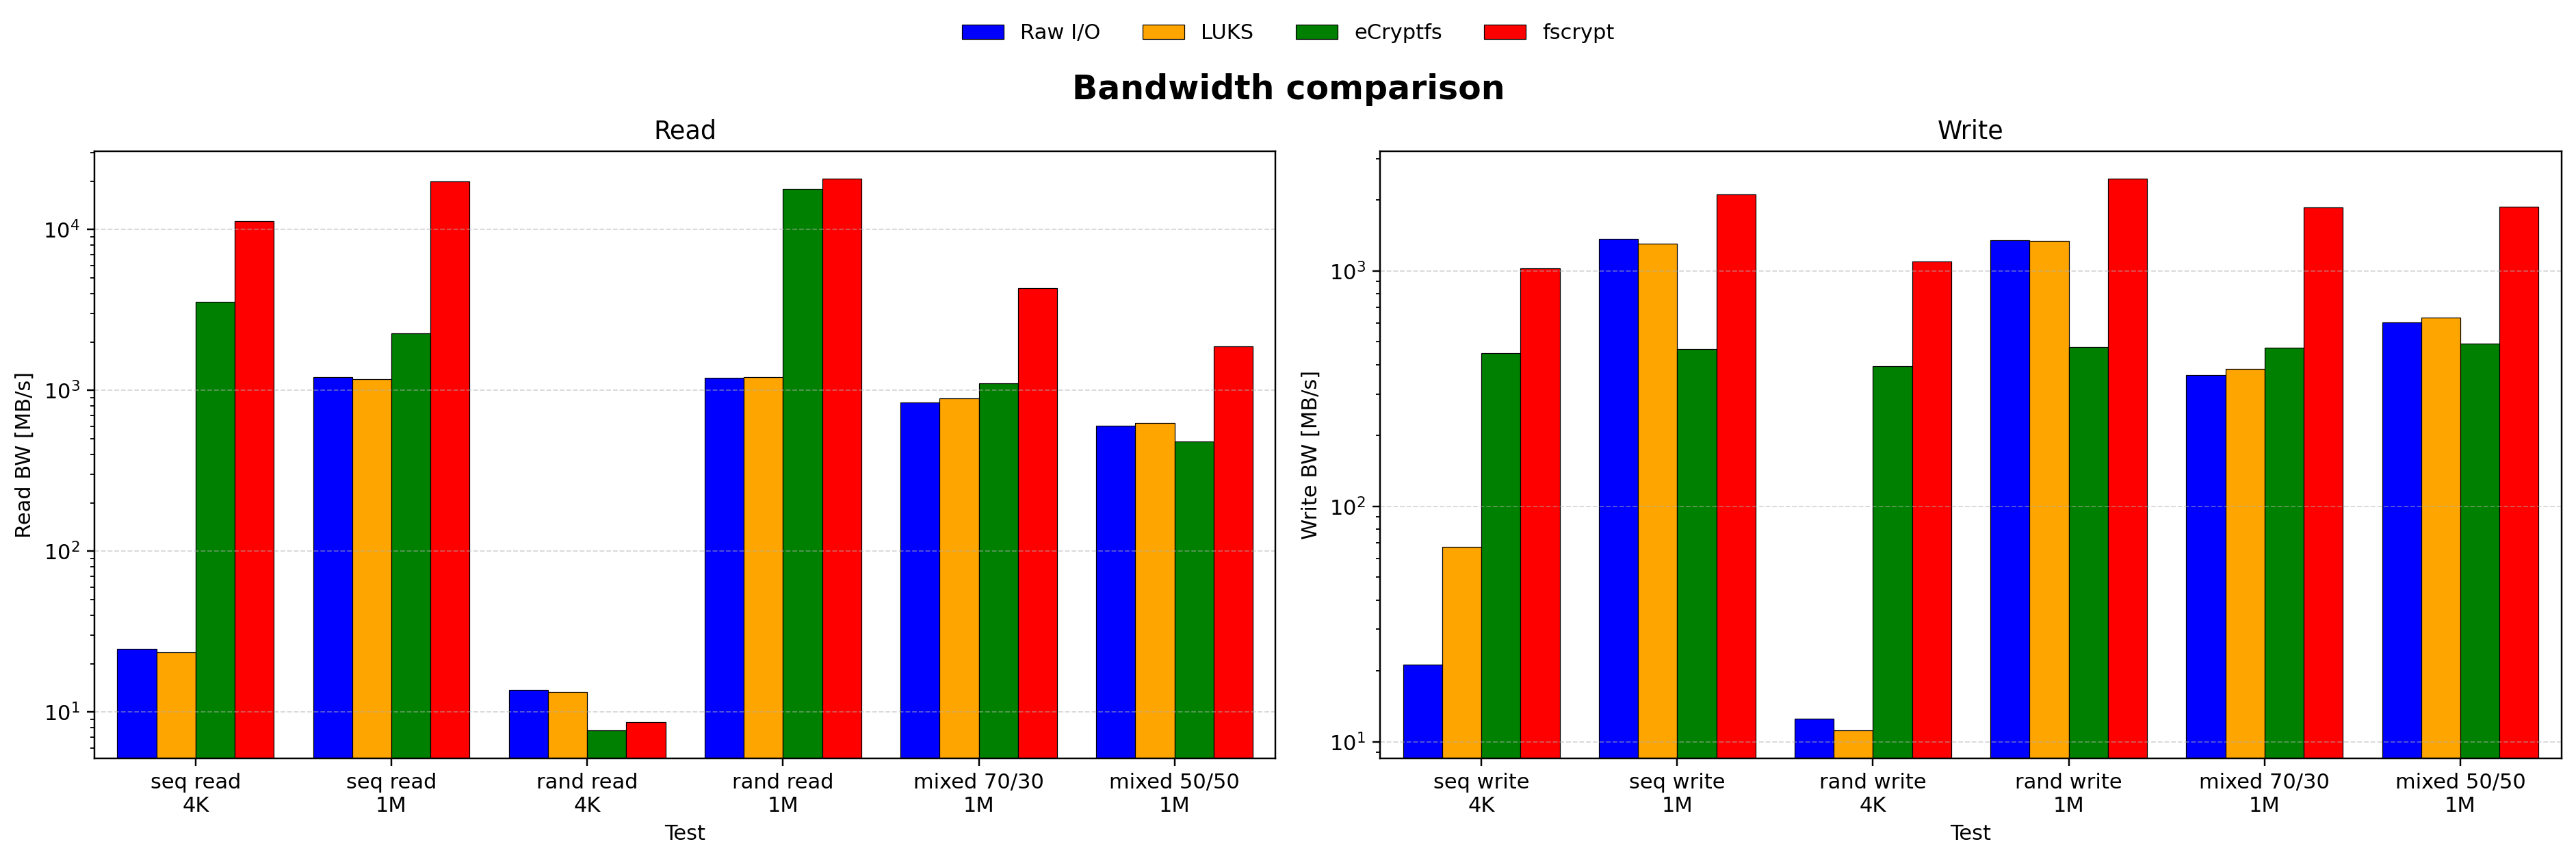
\includegraphics[width=\linewidth]{fio_summary_plots/fio_summary_bandwidth.png}
    \caption{Wykres przepustowości poszczególnych mechanizmów szyfrowania dla kolejnych
    testów wydajności.}
    \label{fig:fio_bandwidth}
\end{figure}

\begin{figure}[H]
    \centering
    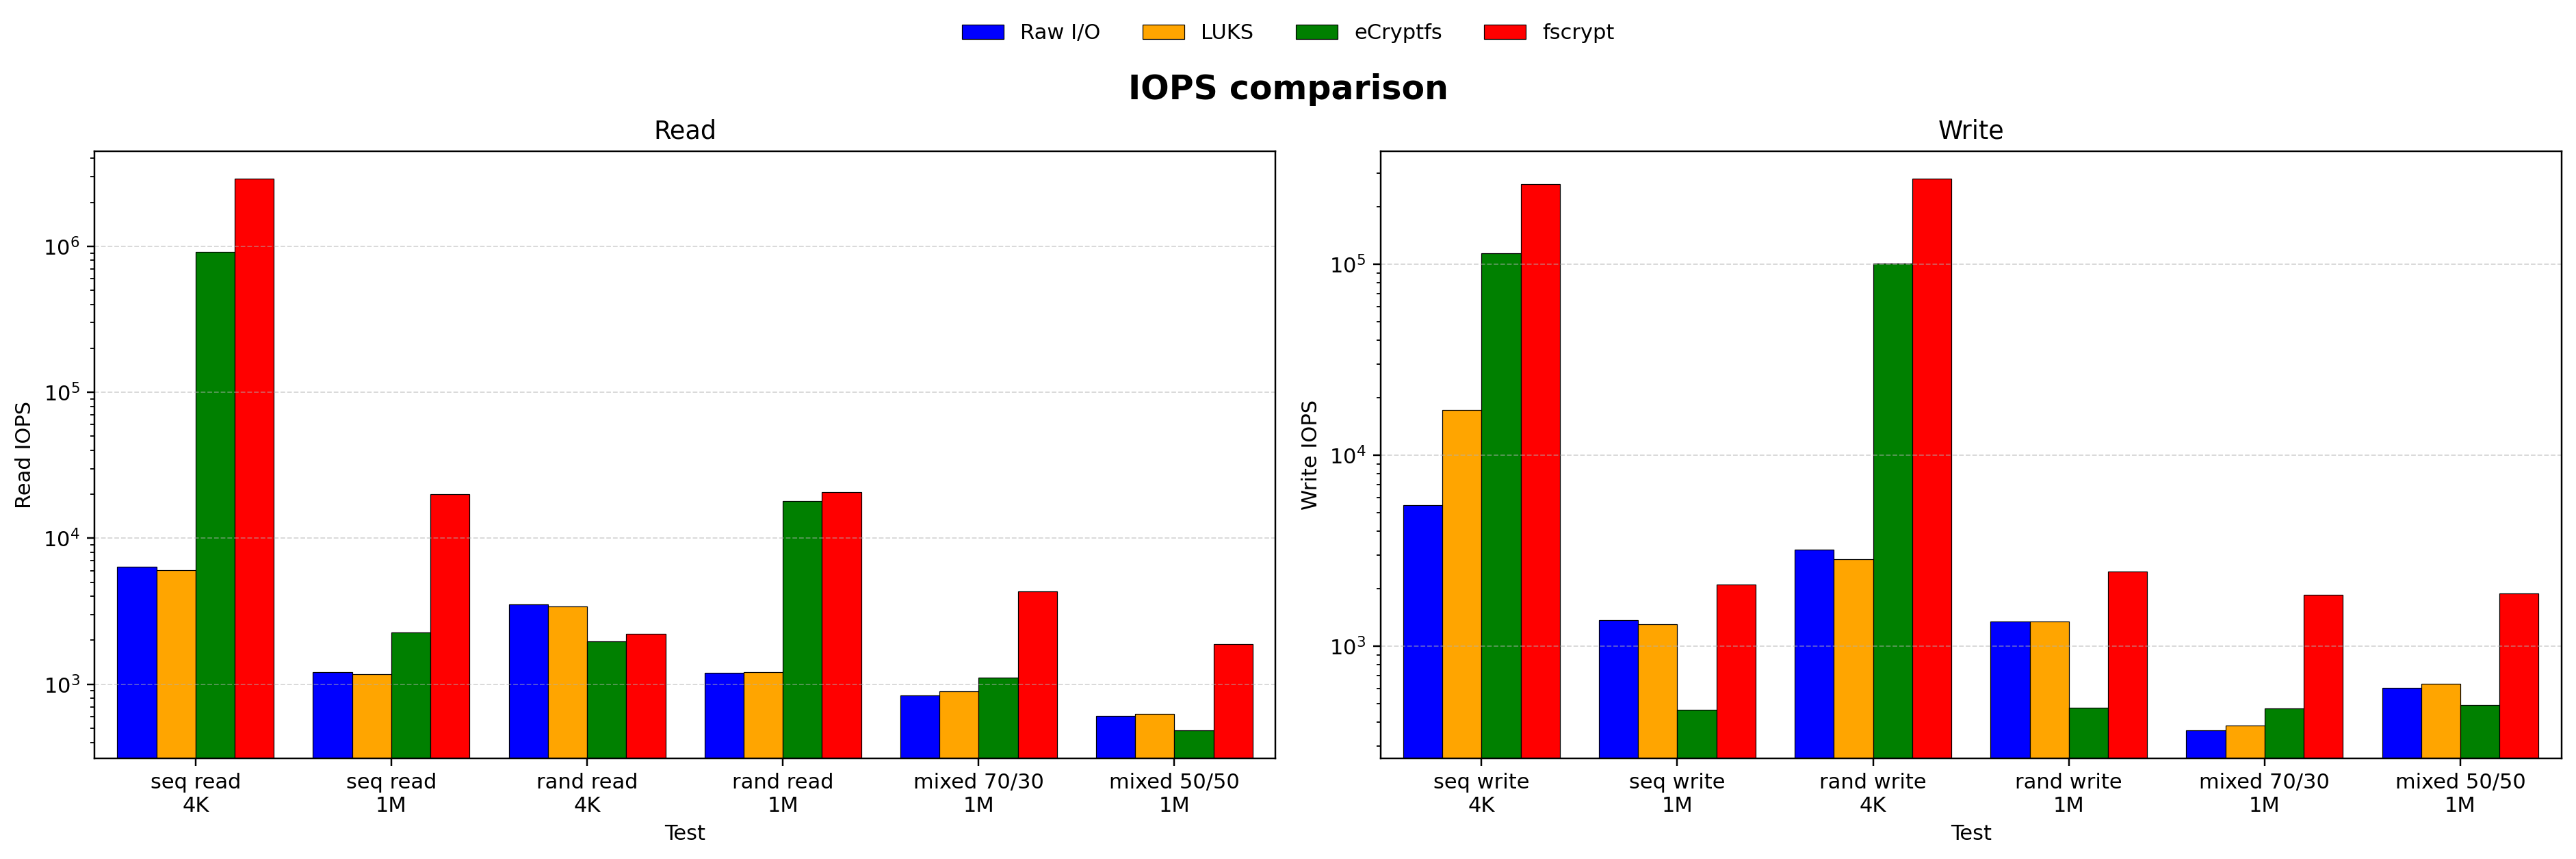
\includegraphics[width=\linewidth]{fio_summary_plots/fio_summary_iops.png}
    \caption{Wykres ilości operacji wejścia i wyjścia na sekundę poszczególnych mechanizmów
    szyfrowania dla kolejnych testów wydajności.}
    \label{fig:fio_iops}
\end{figure}

\begin{figure}[H]
    \centering
    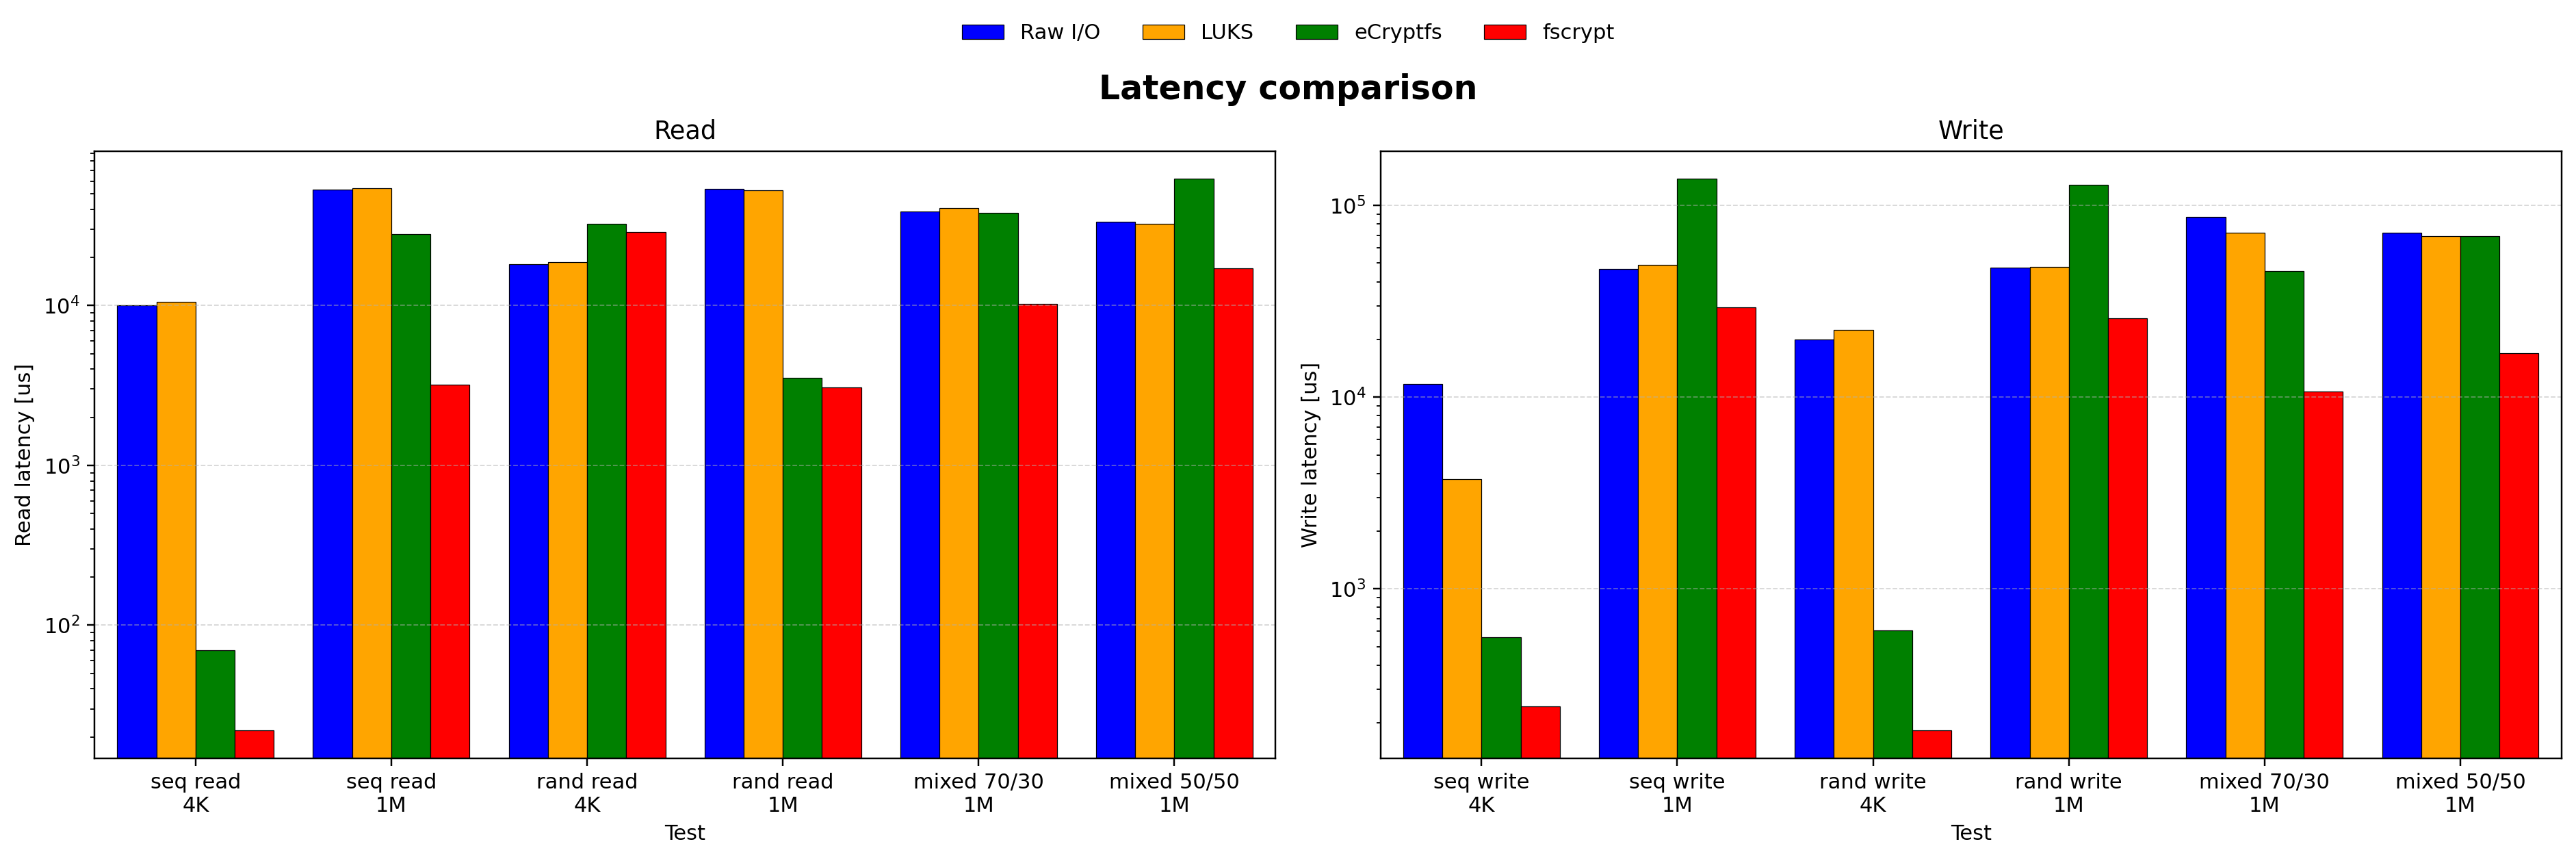
\includegraphics[width=\linewidth]{fio_summary_plots/fio_summary_latency.png}
    \caption{Wykres opóźnienia dla poszczególnych mechanizmów szyfrowania dla kolejnych testów
    wydajności.}
    \label{fig:fio_latency}
\end{figure}

\begin{figure}[H]
    \centering
    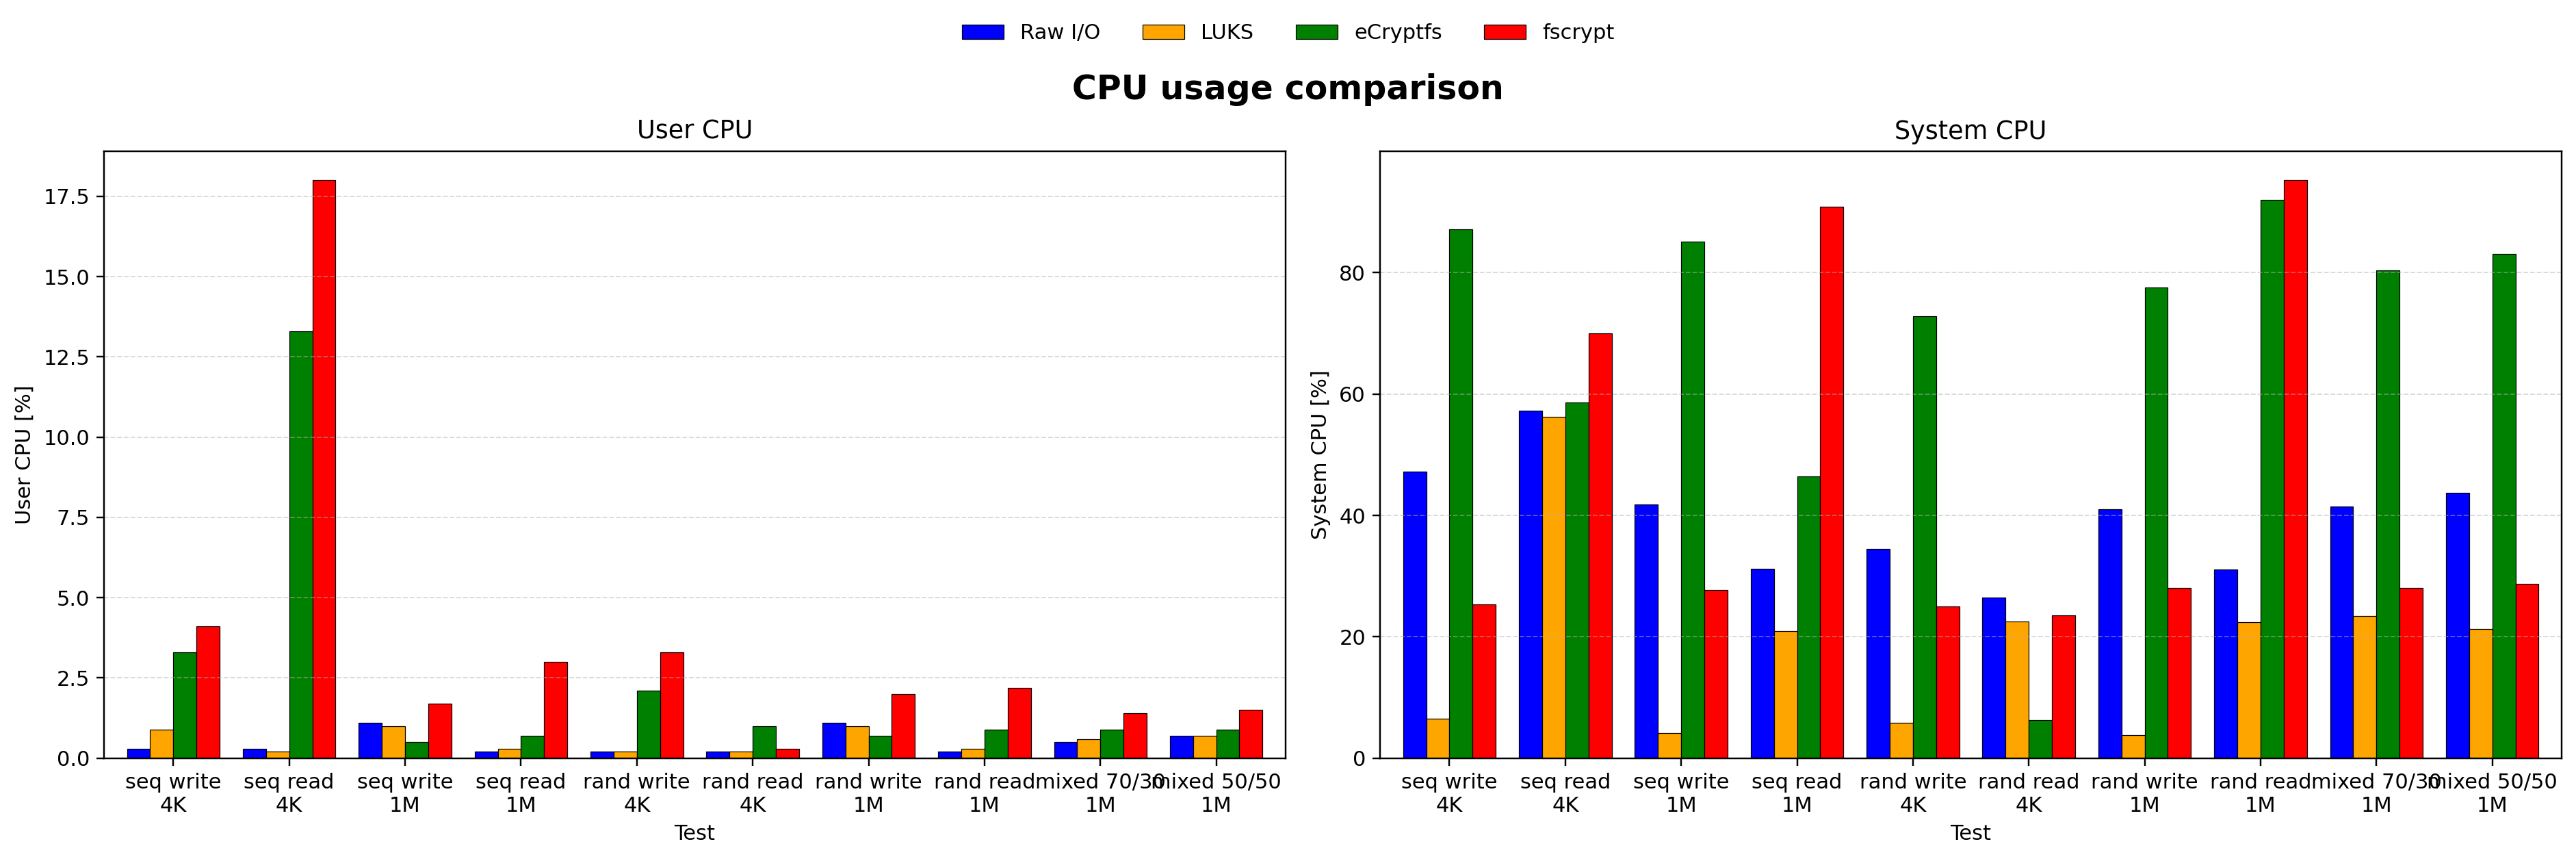
\includegraphics[width=\linewidth]{fio_summary_plots/fio_summary_cpu.png}
    \caption{Wykres zużycia zasobów CPU dla poszczególnych mechanizmów szyfrowania dla kolejnych
    testów wydajności.}
    \label{fig:fio_cpu}
\end{figure}

\subsubsection{Wnioski}

W przypadku wyników otrzymanych dla fscrypt oraz eCryptfs, warto zwrócić uwagę na wykorzystanie
pamięci podręcznej w testach. Pomimo zastosowania flagi \texttt{invalidate=1} w konfiguracji
testów \texttt{fio} oraz czyszczenia bufora jądra przed każdym uruchomieniem benchmarku przy
użyciu poleceń \texttt{sync} oraz \texttt{echo 3 > /proc/sys/vm/drop\_caches}, wyniki dla
fscrypt i eCryptfs wskazują na silny wpływ pamięci RAM.
Dla fscrypt i eCryptfs odczyt danych osiąga przepustowość rzędu kilku, bądź kilkunastu
gigabajtow na sekundę. Otrzymane wartości znacznie przewyższają możliwości wykorzystanego
dysku SSD (około 1200 MB/s dla operacji bez szyfrowania). Wartości rzędu kilkunastu GB na
sekundę wskazują, na przechowywanie danych w pamięci RAM oraz bezpośredni z niej odczyt.

Natomiast wyniki otrzymane dla LUKS są bardzo zbliżone do wyników bez szyfrowania. Warto
zauważyć, że zużycie CPU jest bardzo niskie w trybie systemowym w porównaniu do pozostałych
metod szyfrowania. W testach mieszanych (70\%R/30\%W oraz 50\%R/50\%W), LUKS i brak szyfrowania
osiągają zbliżone wyniki w granicach, co potwierdza spójność wyników dla tego mechanizmu.

\subsection{Podsumowanie}
Wyniki benchmarków pozwalają stwierdzić, że LUKS jest mechanizmem szyfrowania o najmniejszym
narzucie porównując z wydajnością bez szyfrowania, przy jednoczesnym bardzo niskim zużyciu CPU.
eCryptfs niesie za sobą znaczący narzut obliczeniowy (CPU sys powyżej 80\%) oraz obniżoną
przepustowość dla dużych operacji, pomimo że wyniki dla małych bloków są zawyżone na wskutek
buforowania danych. Wyniki fscrypt w zakresie operacji odczytu są silnie powiązane z
wykorzystaniem pamięci cache i nie odzwierciedlają wydajności dyskowej. Jedynie wyniki zapisu
oraz losowego odczytu przedstawiają realne osiągi oraz wydajność mechanizmu.
Mimo zastosowania sposobów czyszczenia pamięci podręcznej, fscrypt skutecznie
ponownie wypełnia cache podczas operacji, co uniemożliwia wiarygodny pomiar wydajności
dyskowej dla tego mechanizmu w zastosowanej konfiguracji testów.




\paragraph{Operacje na małych blokach (4K) kontra dużych blokach (1M).}
We wszystkich mechanizmach przepustowość wyrażona w MB/s dla bloków 4K jest drastycznie
niższa niż dla bloków 1M, co wynika z dominacji opóźnienia dyskowego przy małych operacjach.
Dla Raw I/O sekwencyjny zapis 4K daje 21,29 MB/s, podczas gdy dla 1M wynosi 1\,369,96 MB/s.
LUKS zachowuje tę proporcję, natomiast fscrypt i eCryptfs wykazują tutaj efekty bufora i nie
odzwierciedlają rzeczywistej wydajności dyskowej.


\end{document}
